\begin{frame}


    \begin{columns}[T]
        \begin{column}{0.5\textwidth}
            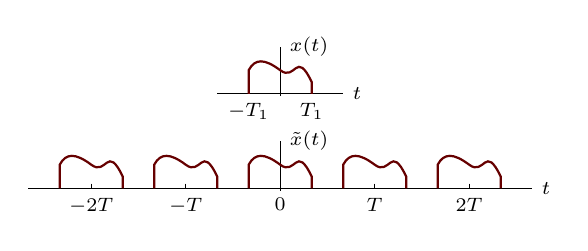
\begin{tikzpicture}[every node/.style={font=\scriptsize}, x=0.4cm, y=0.3cm]
	\def\T1{1cm}		
	\def\T{3}
	\draw (-2, 0) -- (2,0)  node [anchor=west] {$t$};
	\draw (0, -0.1) -- (0, 2) node [anchor=west] {$x(t)$};
	\def\pulse{

		--++(0,1) .. controls ++(0.2,0.5) and ++(-0.5,0.5) .. ++(1,0) .. controls ++(0.5,-0.5) and ++(-0.5,1.4) .. ++(1,-0.5) -- ++(0,-0.5)
	}
	\draw[thick, red!40!black] (-1,0) \pulse;
	\node at (-1,0) [anchor=north] {$-T_1$};
	\node at (1,0) [anchor=north] {$T_1$};
	
	\begin{scope}[yshift = -1.2cm]
		\draw (-8, 0) -- (8,0)  node [anchor=west] {$t$};
		\draw (0, -0.1) -- (0, 2) node [anchor=west] {$\tilde{x}(t)$};	
		\foreach \x/\l in {-2/-2T, -1/-T, 0/0, 1/T, 2/2T}	
		{
			\draw[thick, red!40!black] (\x*\T -1, 0) \pulse;
			\draw (\x*\T, 0.2) -- ++(0, -0.2) node [anchor=north] {$\l$};
		}		
	
	\end{scope}
	
\end{tikzpicture}      
%            \vspace{-0.5cm}
            \begin{align*}
                \tilde{x}(t) &= \sum_{k=-\infty}^{\infty}a_ke^{jk\omega_0 t},\quad \omega_0 =\frac{2\pi}{T}\\
                a_k &= \frac{1}{T}\int_{-T/2}^{T/2}\tilde{x}(t)e^{-jk\omega_0 t}dt.
            \end{align*}
            As $\tilde{x}(t) = x(t)$ for $|t| < T/2$, and also, as $x(t) = 0$ outside this interval,
            \begin{equation*}
                a_k = \frac{1}{T}\int_{-T/2}^{T/2}x(t)e^{-jk\omega_0 t}dt = \frac{1}{T}\int_{-\infty}^{\infty}x(t)e^{-jk\omega_0 t}dt.
            \end{equation*}
        \end{column}
        \begin{column}{0.5\textwidth}
            Defining the envelope $X(j\omega)$ of $Ta_k$ as        
            \begin{equation*}
                X(j\omega) = \int_{-\infty}^{\infty}x(t)e^{-j\omega t}dt,
            \end{equation*}
            we have, for the coefficients $a_k$, 
            \begin{equation*}
                a_k = \frac{1}{T}X(jk\omega_0).
            \end{equation*}
            Combining and expressing $\tilde{x}(t)$ in terms of $X(j\omega)$
            \begin{equation*}
                \tilde{x}(t) = \sum_{k=-\infty}^{\infty} \frac{1}{T}X(jk\omega_0)e^{jk\omega_0 t},
            \end{equation*}        
            or, as $\omega_0 =2\pi/T$    
            \begin{equation}
                \label{eq:xtildet_with_ft}
                \tilde{x}(t) = \frac{1}{2\pi}\sum_{k=-\infty}^{\infty} X(jk\omega_0)e^{jk\omega_0 t}\omega_0.
            \end{equation}             
        \end{column}        
    \end{columns}
\end{frame}


\begin{frame}
    \begin{tikzpicture}[every node/.style={font=\scriptsize}, x=1cm, y=1cm]
	\draw (-2, 0) -- (6,0)  node [anchor=west] {$\omega$};
	\draw (0, -0.1) -- (0, 3.5) node [anchor=west] {$X(j\omega)e^{j\omega t}$};

% \draw (-3.5,1.5) .. controls (-2,3) and (-0.5,2) ..  .. controls (2, 2) and (2, 3) .. (3,1) ;


\draw[pattern=north west lines, pattern color=red!20!white] (2, 0)  node [anchor=north] {$k\omega_0$} rectangle (3, 2.5) ++(0,-2.5) node [anchor=north] {$(k+1)\omega_0$} ;
\draw  plot[smooth, tension=.7] coordinates {(-1.5,2.8) (0,3) (2,2.5) (4.5,1) (5.5,1)};

\draw[dashed] (2, 2.5) -- ++(-2,0) node[anchor=east] {$X(kj\omega_0)^{jk\omega_0 t}$};
\draw[latex-] (2.5,1) -- ++(0.6,-0.4) node [anchor=west, text width=2cm] {Area =\\$X(kj\omega_0)^{jk\omega_0 t}\omega_0$};
\end{tikzpicture}\par
    As $T\rightarrow \infty$, $\tilde{x}(t)$ approaches $x(t)$, and consequently, Eq.~\ref{eq:xtildet_with_ft} becomes a representation of $x(t)$. Furthermore, as $\omega_0 \rightarrow 0$ as $T \rightarrow \infty$, and the right-hand side of  Eq.~\ref{eq:xtildet_with_ft} passes to an integral. As $\omega_0 \rightarrow 0$, the summation converges to the integral of $X(j\omega)e^{j\omega t}$.
    
    \begin{tikzpicture}[remember picture,overlay]
        \node[draw=blue!50, fill=blue!10, inner sep=2pt,outer sep=2pt, rounded corners=0.1cm, anchor=north east, yshift=0cm, xshift=-1cm, text width=5cm]  at (current page.north east) {
            \begin{equation*}
                \tilde{x}(t) = \frac{1}{2\pi}\sum_{k=-\infty}^{\infty} X(jk\omega_0)e^{jk\omega_0 t}\omega_0.
            \end{equation*}
        Inverse Fourier transform:
        \begin{equation*}\label{eq:ift}
            x(t) = \frac{1}{2\pi}\int_{-\infty}^{\infty}X(j\omega)e^{j\omega t} d\omega.
        \end{equation*}
        Fourier transform or Fourier integral:
        \begin{equation*}\label{eq:ft}
            X(j\omega) = \int_{-\infty}^{\infty}x(t)e^{-j\omega t} dt.
        \end{equation*}
        } ;
    \end{tikzpicture}
\end{frame}